Questions 1 and 2 ask you to design a Deterministic Finite-State Automaton (DFA). You are also required to indicate the meaning of each state. Here is an example to show you what we mean by this, taken from an old assignment. The question was:

\begin{quote}
\it
  Design a  deterministic finite-state  automaton (DFA) that  accepts exactly  the strings
  over the alphabet $\{ \verb@A@, \verb@B@, \ldots, \verb@Z@ \}$ that contain at least one
  \verb@C@, at  most two $O$, and  where every $D$  comes before every $E$.  For instance,
  your DFA should accept the strings
  \begin{itemize}
  \item ACCORDEON
  \item CHOCOLATE
  \item CROCODILE
  \item SCALD
  \item SCALE
  \end{itemize}
  but not the strings
  \begin{itemize}
  \item ADRIAN (it doesn't contain the letter \verb@C@)
  \item COLONIZATION (there are three \verb@O@s)
  \item MANACLED (there is an \verb@E@ before a \verb@D@)
  \item BEWARETHEKOMODODRAGON (all of these at the same time)
  \end{itemize}
  Clearly indicate  the meaning of each  state. Hint: there are  three separate conditions
  accepted strings must meet; states will need to  encode whether or not they are met. You can label an edge with the word ``else'' to indicate it would contain every character that does not appear on another edge leaving from the same state. For instance, if a state has outgoing edges labeled ``A'', ``B'', ``E'', ``P'' and ``else'', then ``else'' stands for ``C, D, F, G, H, I, J, K, L, M, N, O, Q, R, S, T, U, V, W, X, Y, Z''.Our
  solution uses 13 states.
\end{quote}

\noindent The solution, and the explanation about the meaning of each state are listed below:
\begin{quote}
\it
  Here is a DFA that works. We used 14 states instead of 13 because having two ``garbage''
  states allows the DFA to be drawn without edges crossing. The idea is that we have three
  separate conditions to check for:
  \begin{itemize}
  \item Whether or  not a ``C'' was seen. The  states in the left half of  the picture are
    those for  which no  ``C'' has  yet been  seen. The states  in the  right half  of the
    picture are those for which a ``C'' has been seen.

  \item Whether or  not a ``E'' was  seen. The states in  the top half of  the picture are
    those for  which no  ``E'' has yet  been seen. The  states in  the bottom half  of the
    picture are those for which a ``E'' has  been seen (and hence seeing a ``D'' will lead
    the DFA to one of the garbage states).

  \item Whether we have seen no ``O'', one  ``O'' or two ``O''s. These states are drawn in
    ``layers'': the  outside rectangle  contains the  states for which  no ``O''  has been
    seen, the middle rectangle contains the states for which a single ``O'' has been seen,
    and the inner rectangle contains the states  for which two ``O''s have been seen. Once
    the DFA reaches a state where two ``O''s have been seen, any further ``O'' leads it to
    a garbage state.
  \end{itemize}
  Twelve  of  the  fourteen  states  encode  all  possible  combinations  of  these  three
  conditions.  The  remaining two  are  garbage  states that  are  used  when one  of  the
  requirements are violated (three or more ``O''s, or a ``D'' after an ``E'') and it is no
  longer possible for the DFA to accept the input string.
  \begin{center}
    \leavevmode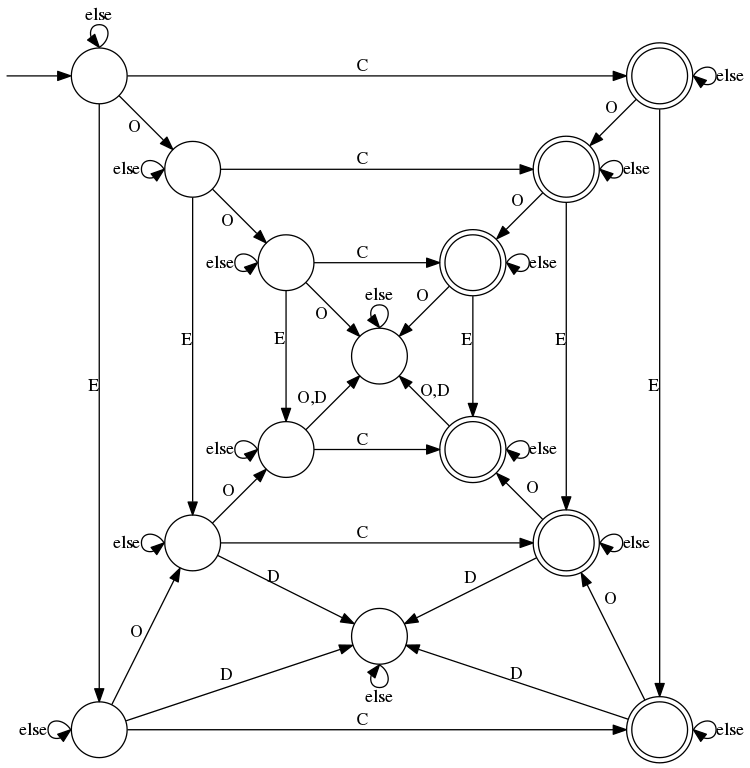
\includegraphics[width=5in]{images/dfa-CODE.png}
  \end{center}
\end{quote}
